% \gls{due}
% \nomenclature[psi]{$\ket{\psi}$}{funzione d'onda}

\section{A Brief History of Neural Networks}
% \label{sec:history-nn}
% % \Glspl{set}

The term \textit{Neural Network} refers to the attempt of defining a mathematical view of the structure of the human brain, aiming at emulating it and transposing the logical functioning and the learning capabilities into computational models.

The very first attempt of studying the biological brain and its neural activity in terms of formal logic is attributed to McCulloch and Pitts,\cite{mcculloch1943logical} who proposed that neurons could be represented as simple binary devices, whose key aspects are:

\begin{itemize}
    \item \textbf{Logical Units:} neurons are basic units with an on/off switch, allowing them to describe neural activi`ty using the language of logic (i.e. logical propositions like \textit{AND}, \textit{OR}...).
    \item \textbf{Threshold:} neurons "fire" only when a certain threshold of input is met.
    \item \textbf{Links:} like synapses, links connect the logical units from the input to the output.
\end{itemize}

This basic understanding of neural processes influeced later developmentes in neuroscience and artificial intelligence, bringing Rosenblatt to produce the \textit{Perceptron}: a single layer neural network that, upon previous work from McCulloch and Pitts, introduced:

\begin{itemize}
    \item \textbf{Weights:} every connection has a weight, that is added to the input received.
    \item \textbf{Learning mechanism:} introduces a learning algorithm where the weights of the connections are adjusted based on errors in the output.
\end{itemize}

This linear architecture allows to generalize the classification tasks, using probabilistic rules that could perform nontrivial tasks like pattern recognition and information organization.

\begin{figure}[ht]
    \centering
    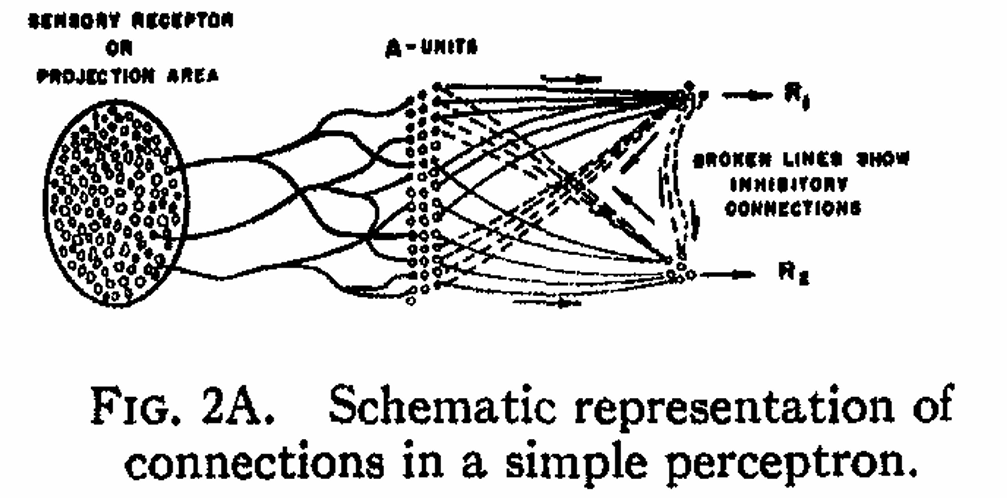
\includegraphics[width=0.5\textwidth]{images/perceptron.png}
    \caption{The perceptron architecture.}
    \label{fig:perceptron}
\end{figure}

Neural networks have evolved dramatically over the decades

The enthusiasm was enormous and the field of cybernetics was born: however, it didn’t take long for researchers to uncover the limitations of single-layer networks. Minsky's and Papert's demonstrated the limitations of the perceptron—that is, that certain classes of functions were simply out of reach for these early models (for example, the logical XOR function)—interest quickly waned. \cite{minsky1969perceptrons}
This realization contributed to a period of reduced enthusiasm for neural network research, often referred to as the “AI Winter.”

Interest was revived in the 1980s with the introduction of the backpropagation algorithm \cite{rumelhart1986learning}, which made it possible for deeper architectures to learn more complex functions. The core idea was to train neural networks by propagating the error from the output layer backward through the network layers; this approach allows the network to adjust its internal weights based on the error itself, so that it could "learn" using gradient descent to minimize the error function, changing the weights individuating the contribution of each neuron in constructing the output.

Although early progress was hampered by hardware constraints, continuous incremental improvements over the following decades, combined with advances in parallel computing, eventually paved the way for the deep learning revolution we see today \cite{goodfellow2016deep}.

By the early 2010s, the impact of Convolutional Neural Networks (CNNs) on computer vision tasks \cite{krizhevsky2012imagenet} highlighted the benefits of large datasets, GPU-based parallel training, and increasingly sophisticated network designs. At the same time, improvements in Recurrent Neural Networks (RNNs)—especially with LSTM \cite{hochreiter1997long}—opened up new possibilities in sequence modeling, including areas like language translation and speech recognition. These advancements ultimately set the stage for the development of Large Language Models (LLMs), particularly after the introduction of the Transformer architecture \cite{vaswani2017attention}.


\section{The Transformer Architecture}
\label{sec:transformer-architecture}

The introduction of the Transformer by Vaswani et al. \cite{vaswani2017attention} marked a clear departure from traditional recurrent and convolutional models. The focus of the original research was on translation tasks, by leaning heavily on a \textbf{self-attention} mechanisms which allows the model to weigh the importance of different words in a seuqence of words, taking into account the relationship to eacht ore.

\begin{figure}[t]
    \centering
    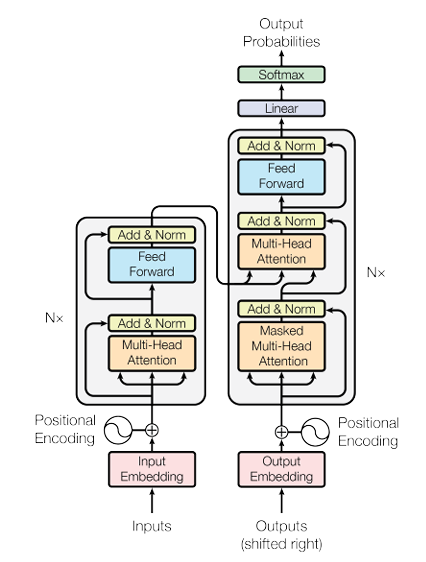
\includegraphics[width=0.5\textwidth]{images/transfomer-architecture.png}
    \caption{The Transformer architecture.}
    \label{fig:transfomer}
\end{figure}

The Transformer architecture consists of two main parts: an \textbf{encoder} and a \textbf{decoder}, each built from multiple layers that implement multi-head self-attention alongside feed-forward networks, which can be visualized in \ref{fig:transfomer}:

\begin{enumerate}
    \item \textbf{Encoder:} it converts an input sequence (e.g., a sentence) into a series of representations that capture the contextual meaning of the input. Within each encode layer, a sub-layer allows every token in the input to consider the influence of every other token.
    \item \textbf{Decoder:} it uses the encoder’s representation along with other inputs to generate a target sequence using a masking mechanism (i.e. predicting the next token is only decided to previous tokens, and not future ones).
\end{enumerate}

\textit{Positional encoding} is another breakthrough of this paper, integrated in both parts, which compensates for the lack of sequence awareness. It incorporates information about the order of tokens in a sequence. Since these models process tokens in parallel rather than sequentially, positional embeddings are essential for conveying information about the order of tokens.

Each of these parts can be used independently, depending on the tasks: encoder-only models are good for tasks that require understanding of the input, such as sentence classification; decoder-only models are good for generative tasks such as text generation.
Encoder-decoder models (called sequence-to-sequence models) are used for generative tasks that require an input, such as translation or summarization.



\section{Transformers as Language Models}
In recent applications, the Transformer model have been trained as \textit{language models} meaning they have been trained on large amounts of raw text in a self-supervised fashion, which is a type of training in which the objective is automatically computed from the inputs of the model.

This type of models develop a statistical understanding of the language it has been trained on, but it’s not very useful for specific practical tasks. Because of this, the general pretrained model then goes through a process called \textit{transfer learning}. During this process, the model is fine-tuned in a supervised way — that is, using human-annotated labels — on a given task.

An example of a task is predicting the next word in a sentence having read the previous words. This is called causal language modeling because the output depends on the past and present inputs, but not the future ones.

Training is a foundamental step in the adoption and implementation of a language model. The learning capacity of LLMs are generally dived into:\cite{liu2024understanding}

\begin{enumerate}
    \item \textbf{Pre-training:} it is the first stage in training an LLM, where the model learns general linguistic patterns, facts and knowledge from a vast corpus of text. It is the act of training a model from scratch: the weights are randomly initialized, and the training starts without any prior knowledge. Tecniques of pre-training phase are:
    \begin{itemize}
        \item \textit{Masked language modeling}, used in decoder-models, where certain words are masked and the model learns to predict them.\cite{devlin2019bert}
        \item \textit{Causal language modeling}, used in encoder-only models like GPT,\cite{brown2020language} where the model predicts the next word in a sequence.
    \end{itemize}
    \item \textbf{Fine-tuning:} after pre-training, the model undergoes a further training on a smaller, task-specific dataset to improve performance for particular and domain-specific applications. Types of fine-tuning are:
    \begin{itemize}
        \item \textit{Supervised fine-tuning} is used to train models on labeled data, such as question-answering datasets.
        \item \textit{Instruction tuning} involves training the model on a dataset of input-output pairs, where each input is phrased as an instruction and the output is the desired response. Most ready-to-use models are instruct-tuned, as they have improved generalization and natural responses. An example can be seen in Table \ref{tab:instruction-tuning}.
        \item \sloppy{\textit{Parameter-Efficient fine-tuning (PEFT)}, methods like \textit{Low-Rank Adaption (LORA)}\cite{hu2021lora} are innovative techniques that reduce the number of parameters to train, thus reducing computaional costs.}
    \end{itemize}
\end{enumerate}

\begin{table}[b]
    \centering
    \renewcommand{\arraystretch}{1.3}
    \begin{tabularx}{\textwidth}{|X|X|X|}
        \hline
        \textbf{Instruction} & \textbf{Input (optional)} & \textbf{Expected Output} \\
        \hline
        Translate this sentence into Spanish & "Hello, how are you?" & "Hola, ¿cómo estás?" \\
        \hline
        Summarize the text in one sentence & "The global economy is facing uncertainty due to inflation and geopolitical issues." & "The global economy is unstable due to inflation and geopolitics." \\
        \hline
        Explain how photosynthesis works to a 5-year-old & \textit{No input} & "Plants use sunlight to make food, like how we eat to get energy!" \\
        \hline
    \end{tabularx}
    \caption{Examples of Instruction Tuning}
    \label{tab:instruction-tuning}
\end{table}

Generally, the strategy to achieve better performance is by increasing the models’ sizes as well as the amount of data they are pretrained on, but higher performances lead to higher resources intensive trainings. This is why different strategies have been developed to achieve good performances without the need of training models.


% \sloppy{\section{Prompt Engineering and RAG}}
\label{sec:key-techniques}


\section{Challenges and Limitations of LLMs}
\label{sec:challenges-llms}


\section{Summary}
\label{sec:background-summary}